\documentclass{supervision}
\usepackage{course}

\Supervision{4}

\begin{document}
  \begin{questions}
    \SetQuestionNumber{12}
    \question \textit{Digital channels, modulation and transmission}
      \begin{parts}
        \part Explain the distinctions between baud rate and bit rate and
          between baseband and broadband.
          \begin{solution}
            Bit rate is just that, the rate at which binary bits can be sent.

            Baud rate is the rate that symbols can be sent. In systems
            where a symbol simply encodes one bit then they are the same but in
            systems where a symbol encodes multiple bits then the baud rate
            will be lower than the bit rate (by a factor equal to the number of
            bits per symbol).

            Baseband is a type of transmission that uses all the bandwidth and
            therefore only a single device can transmit at a time.

            Broadband is a type of transmission that uses a modulated signal,
            using different frequencies to allow multiple devices to transmit
            concurrently.
          \end{solution}

        \part Why is synchronisation not an issue for transmission of
          analogue signals?
          \begin{solution}
            Synchronisation is required when the receiver needs to know where
            the boundaries between data bits are. Since in an analogue signal
            there are no such boundaries it does not need to synchronise.
          \end{solution}

        \part What problem in synchronous transmission is Manchester coding
          designed to solve? Suggest a simpler but possibly more expensive
          way of solving the same problem. Explain why a system which has a
          slow but accurate oscillator would be more suited to asynchronous
          transmission than to synchronous transmission using Manchester
          coding.
          \begin{solution}
            Synchronous transmission requires the sender's clock to be
            synchronised with the reciever's.

            A simpler way of solving this problem is to use start and stop
            bits. The reciever resyncs their internal clock every time one is
            recieved and the clock will be accurate enough to not get out of
            sync within a frame.

             If it has a slow but accurate oscillator then the clock will not
             drift enough to cause the skew between the two clocks to prevent
             communication.

          \end{solution}

        \part List three properties of a sinusoidal waveform which admit
          modulation. Explain the relationship between modulation and shift
          keying.
          \begin{solution}
            Phase, frequency, amplitude.

            Modulation is putting data onto a signal, shift keying is a type of
            modulation that increased or reduces one of the three properties to
            send data.
          \end{solution}
      \end{parts}

    %%%%%%%%%%%%%%%%%%%%%%%%%%%%%
    \section*{Topic 04 - Network}
    %%%%%%%%%%%%%%%%%%%%%%%%%%%%%

    \SetQuestionNumber{14}
    \question \textit{Switching}
      \begin{parts}
        \part Why is switching a practical necessity in large networks? In
          what way is switching a form of multiplexing?
          \begin{solution}
            For a large network it is not feasible for every device to have a
            link to every other device and thus switching of some kind (whether
            circuit switching or packet switching) is required.

            Switching can be thought of as a type of multiplexing as the link
            between an entity and a switch is shared between all over entitys
            that want to communicate with it. In a circuit switched network
            like the phone network then access is on a first-come-first-served
            basis with the link reserved for the duration of the call. In a
            packet switched network the switch will buffer packets.
          \end{solution}

        \part The switching process consists roughly of a demultiplexing
          stage, a routing stage and a remultiplexing stage. For each of the
          following examples of switching, explain what is being
          demultiplexed, what routing decisions are made, and how
          remultiplexing is performed:
          \begin{subparts}
            \subpart packet switching in the postal network;
              \begin{solution}
                When the collection comes in it is demultiplexed into
                individual envelopes and the postcode is used to decide which
                mail van to put it on (routing and remultiplexing).
              \end{solution}

            \subpart packet switching in an Ethernet switch;
              \begin{solution}
                Packets come in and are put in a queue (demultiplexed).
                The switch then looks at the MAC table to determine which
                link to send the packet down and sends it.
              \end{solution}

            \subpart packet switching in an IP router;
              \begin{solution}
                Same as above but the router uses a routing table instead of a
                MAC table.
              \end{solution}

            \subpart circuit switching in the telephone network;
              \begin{solution}
                When a telephone call is made the network establishes a circuit,
                using the area code to route the call.
              \end{solution}

            \subpart wave-division switching in an optical switch.
              \begin{solution}
                \emph{not sure}
              \end{solution}

          \end{subparts}
        \part Switching can improve the efficiency of a network’s link
          utilisation, but may also cause problems. In a packet-switched
          network, two particular problems are increased latency and data
          loss.
          \begin{subparts}
            \subpart For one of the packet-switched examples above, explain
              how latency and loss might occur.
              \begin{solution}
                Every parcel to and from the same place must go through the
                same processing, this can cause delays to parcels.

                \emph{Not sure about loss}
              \end{solution}

            \subpart Using the same example, suggest one way in which latency
              might be improved, and one way in which loss might be reduced.
              \begin{solution}
                Latency could be improved by collecting from the sender for
                large businesses as this could reduce the amount of sorting
                that needs to be done.
              \end{solution}

            \subpart To what extent are the problems of latency and loss less
              significant in circuit-switched networks? Give two
              disadvantages of circuit-switched networks over packet-switched
              networks.
              \begin{solution}
                Latency is bounded by number of links in route. Loss is minimal
                as capacity is reserved.

                Reacting to failure is slower and more difficult and is less
                efficient for bursty transmissions.
              \end{solution}

          \end{subparts}
      \end{parts}

    \SetQuestionNumber{16}
    \question \textit{General routing concerns}
      \begin{parts}
        \part Following are some examples of routing strategies and real
          systems which use them. For each one, suggest one reason why the
          strategy is a good choice, and another in which it might cause
          problems.

          \begin{subparts}
            \subpart flood routing in an Ethernet hub
              \begin{solution}
                If a packet can be delivered it likely will. Since it uses
                every path it will also use the shortest. Flooding is very
                costly in terms of bandwidth as even though a message might
                only have a single destination it will still be sent to all
                hosts.
              \end{solution}

            \subpart random routing in a peer-to-peer file-sharing network
              \begin{solution}
                It is good as clients do not need to have knowledge of the
                network topology but bad because of high packet loss.
              \end{solution}

            \subpart source routing in the road network
              \begin{solution}
                Packets take predictable routes but cannot adapt to changing
                circumstance and client must know entire topology.
              \end{solution}

            \subpart hot potato routing in crowded supermarket aisles (when
              heading for a target grocery shelf)
              \begin{solution}
                \emph{Not entirely sure on the analogy.} One benefit is that
                customers will become more spread out as they seek different
                routes which will ease congestion. A disadvantage is that
                without knowledge of all congested areas a customer may
                walk around and continue to find queues and thus take longer
                to get to there destination aisle.
              \end{solution}

          \end{subparts}
        \part As well as benefits of bounded latency and assured capacity,
          circuit switching allows routing to be performed only once per
          connection, at set-up time. This contrasts with datagram-based
          routing, as commonly used in packet-switched networks, where
          routing is done for each datagram individually.

          \begin{subparts}
            \subpart Outline a set of additions or modifications to TCP/IP
              which would allow routing decisions to be made only once per
              TCP connection. Identify what (if any) other benefits of
              circuit switching your modifications provide, and which ones
              they do not.
              \begin{solution}
                Add a circuit setup and teardown request to the protocol. A
                circuit setup sends a packet like normal but every node stores:
                the source address, the destination address, the incoming link
                and the outgoing link. When the circuit setup packet reaches
                the destination it sends an acknowledgement back (which will
                be routed via the same route since all the nodes will
                match the destination and source addresses).

                The state in the routing table persists until either it
                timeouts or a teardown packet is sent. If the routing table is
                full and a setup circuit packet is sent to it then it will
                reject the packet.
              \end{solution}

            \subpart Do your modifications preserve the reliability
              properties of datagram-based routing? Specifically, the
              property in question is that end-to-end connections can be
              maintained across a catastrophic failure of a router or link,
              assuming that an alternative path through the network exists.
              If they do, explain why. If not, suggest how this could be
              achieved, or explain why your modifications expressly preclude
              it.
              \begin{solution}
                If a node on the circuit fails then the circuit will break and
                the network does nothing to recover from this - it is up to the
                sender to realise that they are not receiving acknowledgement
                packets and request a new circuit.
              \end{solution}


          \end{subparts}
        \part You are required to design a topology discovery protocol for a
          network of switching nodes interconnected by links. There are $n$
          nodes, $l$ links, the maximum degree of any node is $k$ and there
          is a path between any two nodes of not more than $d$ hops. All
          links are bi-directional.

          Each node has a unique identifier of four bytes which it knows.

          \begin{subparts}
            \subpart Outline a protocol (including message formats) for a
              node to learn about its immediate neighbours.
              \begin{solution}
                The node sends a discover packet to its immediate neighbours
                with its own \lstinline|NODE ID|. The neighbours then reply
                with a discovery reply packet with their IDs.
              \end{solution}


            \subpart Design a protocol (including message formats) for
              distributing this information across the network.
              \begin{solution}
                When a node has established the identity of its neighbours it
                floods this to the network. It only floods the neighbours for
                which its own ID is greater than theirs. Since the network
                guarantees that no other node is more than $d$ hops away $d$
                should be used as the TTL.
              \end{solution}

            \subpart Give a bound on the total amount of information which is
              transmitted to ensure that every node acquires complete
              topology information.
              \begin{solution}
                There are $l$ links, each link is flooded once to every other
                node and thus the bound on the total amount of information
                (assuming no retransmission is required) is $O(l*n)$.
              \end{solution}

          \end{subparts}

        \part Consider a Distance-Vector Routing protocol. The routing
          table for node $A$ is expresed in a format where the rows
          indicate the destination and the columns indicate the first
          hop. That is, the number in (row $C$ column $D$) denotes the
          cost of the best currently known path to $C$ that starts with
          $A$ and sending to $D$. The initial table for Node $A$, before
          $A$ has exchanged any routing information with any other node,
          takes the form:

          \begin{table}[h!]
            \centering
            \begin{tabular}{|c|ccc|}
              \hline
              Table for A & B        & C        & D        \\ \hline
              B           & 3        & $\infty$ & $\infty$ \\
              C           & 4        & 1        & $\infty$ \\
              D           & $\infty$ & $\infty$ & 2        \\
              E           & $\infty$ & $\infty$ & $\infty$ \\
              F           & $\infty$ & $\infty$ & $\infty$ \\ \hline
            \end{tabular}
          \end{table}

          \emph{Note that in this initial routing table, $A$ does not know paths
          to any destinations except its immediate neighbours.}

          \begin{figure}[h!]
            \caption{A network topology. Numbers refer to the link-cost of
              indicated link.}
            \label{fig:1}
            \centering
              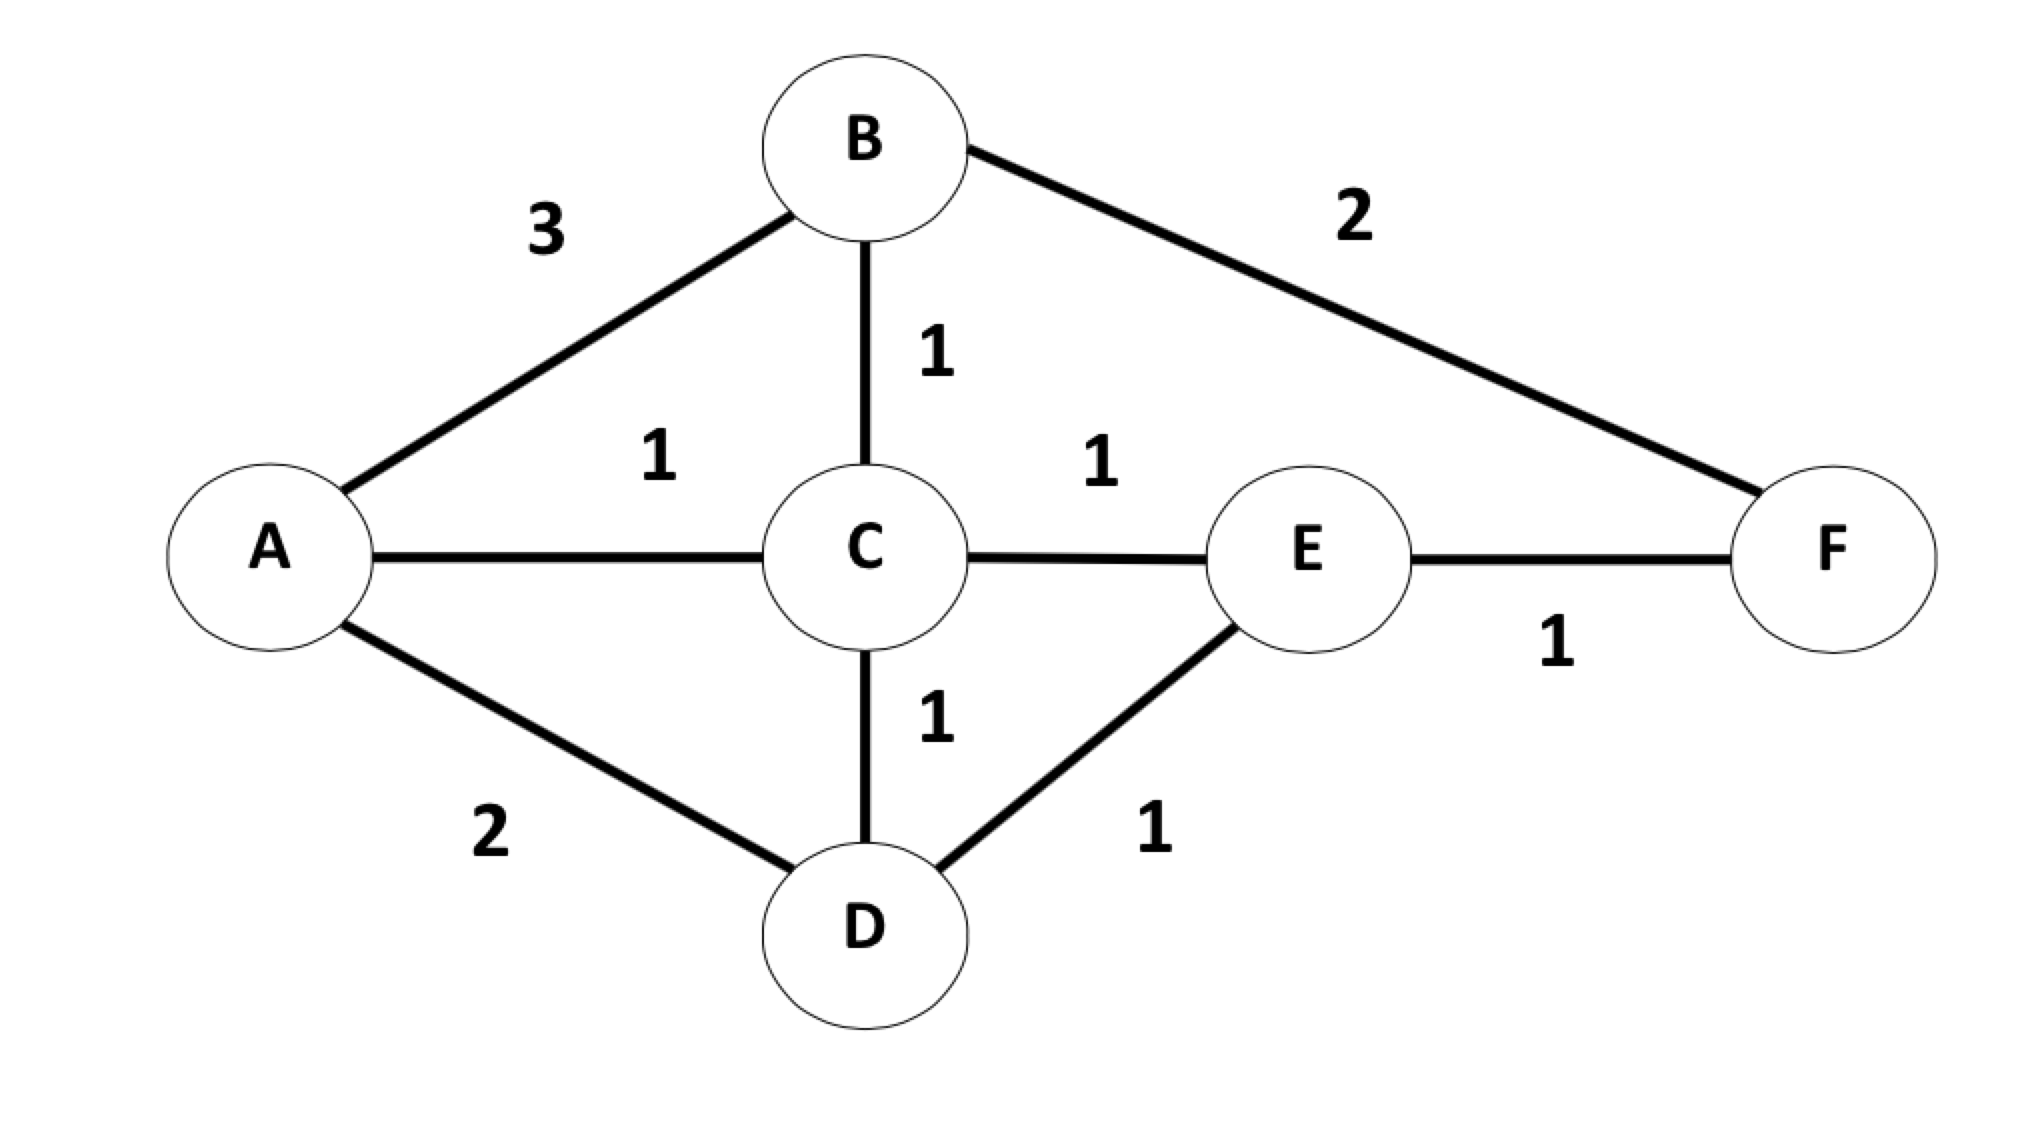
\includegraphics[width=0.75\textwidth]{16-figure-1}
          \end{figure}

          \begin{subparts}
            \subpart After $A$ receives a route update from $B$ ($B$ sends
              its initial table), what are the entries in the routing table
              for $A$?
              \begin{solution}
                \begin{center}
                  \begin{tabular}{|c|ccc|}
                    \hline
                    Table for A & B        & C        & D        \\ \hline
                    B           & 3        & $\infty$ & $\infty$ \\
                    C           & 4        & 1        & $\infty$ \\
                    D           & $\infty$ & $\infty$ & 2        \\
                    E           & $\infty$ & $\infty$ & $\infty$ \\
                    F           & 5        & $\infty$ & $\infty$ \\ \hline
                  \end{tabular}
                \end{center}
              \end{solution}

            \subpart After $A$ receives a route update from $C$ ($C$ sends
              its initial table), what are the entries in the routing table
              for $A$?
              \begin{solution}
                \begin{center}
                  \begin{tabular}{|c|ccc|}
                    \hline
                    Table for A & B        & C        & D        \\ \hline
                    B           & 3        & 2        & $\infty$ \\
                    C           & 4        & 1        & $\infty$ \\
                    D           & $\infty$ & 2        & 2        \\
                    E           & $\infty$ & 2        & $\infty$ \\
                    F           & 5        & $\infty$ & $\infty$ \\ \hline
                  \end{tabular}
                \end{center}
              \end{solution}

            \subpart Assume now that all nodes exchange tables in an
              iterative process until steady-state is achieved. What are the
              steady-state entries in the table for node $A$?
              \begin{solution}
                \begin{center}
                  \begin{tabular}{|c|ccc|}
                    \hline
                    Table for A & B        & C        & D        \\ \hline
                    B           & 3        & 2        & 4        \\
                    C           & 4        & 1        & 3        \\
                    D           & 5        & 2        & 2        \\
                    E           & 5        & 2        & 3        \\
                    F           & 5        & 3        & 4        \\ \hline
                  \end{tabular}
                \end{center}
              \end{solution}
          \end{subparts}

          Now consider the network of Figure \ref{fig:1} and a Link-State
          Routing algorithm.

          \begin{subparts}
            \SetQuestionNumber{4}
            \subpart If $A$ sends a packet to $B$, what path does the packet
              take?
              \begin{solution}
                It goes via $C$.
              \end{solution}

            \subpart If $A$ sends a packet to $F$, what path does the packet
              take?
              \begin{solution}
                It goes to $C$, then to $E$ then reaches its destination.
              \end{solution}

            \subpart Now assume that the link cost for the links $C-E$ and
              $E-F$ both change to $6$. $E$ announces these changes and all
              nodes but $C$ get the update (that is, $C$ still thinks $C-E$
              and $E-F$ are link-cost $1$). Now $A$ sends to $F$, what path
              does the packet take?
              \begin{solution}
                $A$ sends the packet to $C$, $C$ sends the packet to $E$.
                $E$ sends the packet to $F$
              \end{solution}

            \subpart Finally, $C$ gets the new link-weight information and
              now knows that $C-E$ and $E-F$ are link-cost $6$. When $A$
              sends to $F$, what path does it take?
              \begin{solution}
                $A$ sends to $C$ whic sends to $B$ which sends to $F$.
              \end{solution}

          \end{subparts}
      \end{parts}
    \question \textit{Supervision discussion questions}
      \begin{parts}
        \part Compare Forwarding versus Routing

        \part Compare and contrast Link-State Routing with Distance-Vector
          Routing. What are the (information) consistency models of each?
          What information is exchanged?

        \part What makes a fast LPM algorithm? (Longest-Prefix-Match)?

        \part What happens when (packet) fragment loss occurs?

        \part What is the state held by a NAT box? How does a NAT box work
          out its state?

        \part Why do packets tend towards the same path(route) through the
          network?

        \part How does ARP work?

        \part Compare DNS and ARP

        \part Why would I (or wouldn’t I) want to broadcast an ARP response?

        \part How does Gateway ARP do its thing?
      \end{parts}
  \end{questions}
\end{document}
